\documentclass[12pt]{article}
\usepackage{listings} % Include the listings package
\usepackage[T1]{fontenc} % Add the fontenc package with T1 encoding
\usepackage{subcaption}

\PassOptionsToPackage{maxbibnames=99}{biblatex}
\usepackage{./Layout/EngReport}

\setlength{\headheight}{35pt}

\usepackage{indentfirst}
\addbibresource{./Layout/Sources.bib}

\graphicspath{{Images/}}
\onehalfspacing
\geometry{a4paper, portrait, includeheadfoot=true, hmargin=1in, vmargin=1in}

% Adjust Table of Contents spacing for "Appendix X" labels
% This prevents the overlap of "Appendix A", "Appendix B" with titles
\usepackage{tocloft}
\setlength{\cftsubsecnumwidth}{6em}  % Width for subsection numbers (Appendix A)
\setlength{\cftsubsubsecnumwidth}{6.5em}  % Width for subsubsection numbers (Appendix A.A)
\setlength{\cftsubsecindent}{1.5em}  % Indent for subsections
\setlength{\cftsubsubsecindent}{3em}  % Indent for subsubsections

% Configure listings to handle UTF-8 characters properly
\lstset{
	inputencoding=utf8,
	extendedchars=true,
	literate=
	{°}{{$^\circ$}}1
	{α}{{$\alpha$}}1
	{σ}{{$\sigma$}}1
	{∇}{{$\nabla$}}1
	{≈}{{$\approx$}}1
	{≤}{{$\leq$}}1
	{≥}{{$\geq$}}1
	{→}{{$\rightarrow$}}1
	{←}{{$\leftarrow$}}1
	{✓}{{\checkmark}}1
	{✗}{{$\times$}}1
	{—}{{---}}1
	{–}{{--}}1
	{²}{{$^2$}}1
	{₀}{{$_0$}}1
	{₁}{{$_1$}}1
	{₂}{{$_2$}}1
	{ᵀ}{{$^T$}}1
	{·}{{$\cdot$}}1
	{×}{{$\times$}}1
	{ρ}{{$\rho$}}1
	{β}{{$\beta$}}1
	{ε}{{$\varepsilon$}}1
	{∂}{{$\partial$}}1
	{∞}{{$\infty$}}1
	{³}{{$^3$}}1
	{À}{{\`A}}1
	{È}{{\`E}}1
	{Ô}{{\^O}}1
	{Δ}{{$\Delta$}}1
	{É}{{\'E}}1
	{é}{{\'e}}1
	{è}{{\`e}}1
	{ê}{{\^e}}1
	{à}{{\`a}}1
	{â}{{\^a}}1
	{ù}{{\`u}}1
	{û}{{\^u}}1
	{î}{{\^i}}1
	{ï}{{\"i}}1
	{ô}{{\^o}}1
	{ç}{{\c{c}}}1
}


\begin{document}
	\renewcommand{\familydefault}{\rmdefault}
	
	\begin{titlepage}
    \begin{center}
    {\fontsize{40}{48}\selectfont \bfseries Cooling Tower Optimisation} 
    \\\vspace{20pt}
    {\LARGE Task 6 (Group Report)} \\
    \vspace{20pt}
    
    \vfill % Fills the vertical space above the image

        
\includegraphics[width=0.25\textwidth]{Images/cranfield_logo.png}

        \vfill % Fills the vertical space below the image
        \textbf{Pierre BEDRUNE, Martin HARRAMBAT, Clémence-Philomène HINOT, John HOARAU}

        Prepared for March 6, 2026
    \end{center}
\end{titlepage}
	\pagestyle{fancy}
\fancyhf{}
\setlength{\headheight}{35pt}
\renewcommand{\headrulewidth}{0.4pt}
\renewcommand{\footrulewidth}{0.4pt}
\lhead{\large Task 6 (Group Report) \\ Applications of Computational Engineering Design}
\rhead{\large January 6, 2026 \\ Chenonceau Group}
\rfoot{\textbf{Page \thepage}}
\lfoot{}


	
	% Arabic numerals for main content (starts from 1)
	\pagenumbering{arabic}
	
	\fontsize{12}{20}\selectfont{
		
		\begin{abstract}

This report addresses the structural optimisation of a natural-draught cooling tower, modelled as a vertical stack of $m = 10$ conical frustums. 
The objective is to minimise the total lateral surface area, a proxy for construction material cost, 
subject to a fixed internal volume constraint of $V_{\text{target}} = 70{,}320\,\text{m}^3$. 
The equality constraint is handled via a quadratic penalty method, enabling a uniform, solver-agnostic problem formulation.

Three optimisation algorithms are benchmarked: the quasi-Newton Broyden-Fletcher-Goldfarb-Shanno (BFGS) method, 
Particle Swarm Optimisation (PSO), and Simulated Annealing (SA). 
Their performance is evaluated across eight study cases of increasing complexity, ranging from a fixed-height reference case ($D = 9$) 
to a parametric hyperboloidal fit ($D = 3$), 
encompassing variations in dimensionality, initialisation strategy, constraint topology, and physical scaling.

Results demonstrate that NEED TO GET THE FINAL RESULTS 
\end{abstract}

		\pagebreak
		
		\section*{Acronyms}
% Using \section* (with asterisk) to create an unnumbered section

\begin{description}
	\item[BFGS] Broyden-Fletcher-Goldfarb-Shanno
	\item[PSO] Particle Swarm Optimisation
	\item[SA] Simulated Annealing
\end{description}
		\pagebreak
		
	}
	
	\tableofcontents
	\pagebreak
	
	\fontsize{12}{20}\selectfont{
		
		\section{Introduction}

Structural optimisation is a cornerstone of modern computational engineering, enabling the design of lighter, more efficient, and more cost-effective structures. 
Among the most widely studied civil structures in this context is the natural-draught cooling tower, whose hyperboloidal shell geometry presents a rich landscape of continuous, nonlinear optimisation challenges~\cite{mungan1976buckling}. 
Minimising the lateral surface area of such a tower, directly proportional to construction material consumption, while satisfying a strict volumetric capacity constraint is a problem of both theoretical interest and direct industrial relevance.

This report constitutes Task 6 of the Digital Engineering Design Group Project undertaken by Group Chenonceau within the MSc in Computational and Software Techniques in Engineering at Cranfield University. 
The group comprises John Hoarau (Project Lead and Integration), Martin Harambat (BFGS Implementation), Pierre B\'{e}drune (Simulated Annealing), and Cl\'{e}mence-Philom\`{e}ne Hinot (Particle Swarm Optimisation and \LaTeX).

\subsection{Project Context and Progression}

Over the preceding tasks, we as a group progressively built our optimisation competence through a structured sequence of increasingly complex problems. 
In Task 3, two metaheuristic algorithms, Particle Swarm Optimisation (PSO) and Simulated Annealing (SA), were independently developed and validated against
 two canonical benchmarks: the discrete Gear Train Design problem and the multi-objective Two-Bar Plane Truss Design problem. 
Task 4 then introduced a deterministic gradient-based counterpart, the Broyden-Fletcher-Goldfarb-Shanno (BFGS) quasi-Newton method, applied to the same benchmarks to
 enable direct algorithmic comparison. 
Key outcomes included the characterisation of BFGS superlinear convergence properties, the evaluation of noise robustness across all three methods, and the identification 
of the complementary strengths and weaknesses of stochastic versus deterministic approaches.

Task 6 represents the culmination of this progression. For the first time, all three algorithms are deployed together on a single, real-world structural optimisation problem: the minimisation of the lateral surface area of a discretised hyperboloidal cooling tower subject to a fixed volume constraint.

\subsection{Problem Statement}

The cooling tower is modelled as a vertical stack of $m$ conical frustums, yielding a constrained nonlinear programme (NLP) 
in which the decision variables, subsets of the internal radii and section heights, are optimised to minimise the total lateral surface area while preserving a target 
internal volume $V_{\text{target}} = 70{,}320\,\text{m}^3$. The equality constraint is handled via a quadratic penalty method,
 enabling uniform treatment across all three solvers without introducing algorithm-specific constraint logic.

To comprehensively evaluate algorithmic performance, eight study cases of increasing complexity are defined. These range from a fixed-height reference case ($D = 9$ decision variables) 
to a parametric hyperboloidal fit ($D = 3$), encompassing variations in decision variable type, dimensionality, initialisation strategy, constraint topology, and physical scaling.

\subsection{Report Structure}

The remainder of this report is organised as follows. Section 2 presents the mathematical formulation of the cooling tower problem, 
the quadratic penalty methodology, the software architecture, and the rationale behind the eight study cases. 
Section 3 details the three optimisation algorithms and their respective adaptations to this problem. 
Section 4 reports the results across all cases and algorithms. 
Section 5 provides a comparative discussion on convergence behaviour, constraint satisfaction, and computational cost. Finally, 
Section 6 draws conclusions and identifies directions for future work.

\subsection{Statement on the Use of Generative AI}

During the preparation of this work, the authors used ChatGPT (OpenAI) and Claude AI (Anthropic) to assist with code efficiency optimisation and debugging, 
technical writing refinement, and literature review formatting. 
After using these tools, all content was reviewed and edited as needed. 
The authors take full responsibility for the final report's content, analysis, and code functionality.

		\pagebreak
		
		\section{Cooling Tower}

\subsection{Mathematical Problem Formulation and Geometric Parametrisation}

The cooling tower of a nuclear power plant defines a continuous surface optimisation problem over a rotationally symmetric structure. 
To render this tractable computationally, the continuous domain is discretised into a vertical stack of $m$ conical frustums, bounded by $m+1$ horizontal cross-sections (rings). 
Let $z$ denote the vertical axis originating at the tower base, with $z_0 = 0$. 
Each frustum $i \in \{1, \dots, m\}$ is fully characterised by its bottom radius $r_{i-1}$, top radius $r_i$, and section height $h_i$.

The macroscopic engineering objective is to minimise construction material costs, which are directly proportional to the total lateral surface area $A_{\text{total}}$. 
This is subject to a strict equality constraint enforcing a fixed thermodynamic cooling capacity, expressed as a target volume $V_{\text{target}} = 70{,}320\,\text{m}^3$. 
For each frustum $i$, the slant height $s_i$, lateral surface area $A_i$, and volumetric capacity $V_i$ are given by:

\begin{align}
    s_i &= \sqrt{(r_{i-1} - r_i)^2 + h_i^2} \\
    A_i &= \pi (r_{i-1} + r_i)\, s_i \\
    V_i &= \frac{\pi h_i}{3} \left( r_{i-1}^2 + r_{i-1} r_i + r_i^2 \right)
\end{align}

The resulting global problem is formally a constrained nonlinear programme (NLP):

\begin{equation}
    \min_{\mathbf{x} \in \mathcal{D}}\; A_{\text{total}}(\mathbf{x}) = \sum_{i=1}^{m} A_i(\mathbf{x})
    \quad \text{subject to} \quad
    \mathcal{H}(\mathbf{x}) = \sum_{i=1}^{m} V_i(\mathbf{x}) - V_{\text{target}} = 0
\end{equation}

where $\mathbf{x}$ is the decision variable vector, and $\mathcal{D} \subseteq \mathbb{R}^{D}$ is the feasible space defined by the physical boundary conditions.

\subsection{Methodology: Quadratic Penalty Formulation and Search Landscape}

To evaluate the three fundamentally different algorithms, Simulated Annealing (SA), Particle Swarm Optimisation (PSO), and the quasi-Newton BFGS method, on a common, unbiased basis, the equality constraint $\mathcal{H}(\mathbf{x}) = 0$ must be handled uniformly. 
Since SA and PSO are natively unconstrained, and since introducing solver-specific constraint-handling logic would compromise benchmark fairness, the equality constraint is absorbed into the objective via a \textbf{quadratic penalty method}. 

The surrogate objective becomes:

\begin{equation}
    J(\mathbf{x}) = A_{\text{total}}(\mathbf{x}) + \rho \left[\mathcal{H}(\mathbf{x})\right]^2
\end{equation}

where $\rho \gg 0$ is a static scalar penalty weight. A static $\rho$ is deliberately chosen over an adaptive schedule to ensure that all three algorithms operate on an identical, fixed search landscape any dynamic $\rho$ strategy would introduce algorithm-dependent trajectory effects that would confound the performance comparison. 
The chosen value $\rho = 10^3$ was calibrated empirically to ensure that volume violations incur a penalty several orders of magnitude larger than the surface area objective, effectively rendering infeasible solutions non-competitive without distorting the local geometry near the feasible manifold.

This penalty formulation has two notable consequences on the search landscape. 
First, for BFGS, the quadratic term degrades the conditioning of the Hessian approximation in proportion to $\rho$, increasing the curvature of the surrogate near constraint boundaries~\cite{nocedal2006numerical}. 
Second, for SA and PSO, the penalty creates steep regions of high curvature in the search landscape around infeasible points, placing greater demands on the exploration-exploitation balance of each algorithm.

\subsection{Architectural Decoupling and Benchmark Fairness}

A fully decoupled, object-oriented software architecture was implemented around a central \texttt{CoolingTowerProblem} class, which encapsulates the geometric model and all case-specific logic. 
The key design principle is a vector mapping pipeline (\texttt{unpack\_decision\_variables}): all three solvers interact exclusively with an abstract decision vector $\mathbf{x} \in \mathbb{R}^D$, with no knowledge of the underlying physical structure. 
The class internally reconstructs the full radii and heights arrays from $\mathbf{x}$ according to the active case. 
This architecture ensures that the \texttt{solver.py} orchestrator applies each algorithm identically across all eight cases, with no solver-specific preprocessing or constraint logic injected at the call level. 
The result is a genuinely fair, one-to-one algorithmic comparison.

\subsection{Study Cases: Dimensionality and Physical Complexity}

Eight cases were designed to progressively stress-test the algorithms across increasing levels of search space complexity, physical realism, and parametric dimensionality. 
All cases are evaluated against BFGS, SA, and PSO.

\begin{itemize}

    \item \textbf{Case 1: Mandatory Reference Case ($D = 9$):}
    The canonical benchmark. Section heights $h_i$ and boundary radii $r_0 = 39.3\,\text{m}$, $r_m = 27.4\,\text{m}$ are fixed, and the nine inner radii $r_1, \dots, r_9$ constitute the sole decision variables. 
	This low-dimensional, well-conditioned problem serves as the convergence baseline against which all other cases are evaluated.

    \item \textbf{Case 2: Variable Heights ($D = 10$):}
    The radii profile from Case 1 is fixed, and the ten section heights $h_i$ are optimised instead. 
	This isolates the vertical sensitivity of the volume constraint and characterises how each algorithm navigates a height-dominated feasible manifold.

    \item \textbf{Case 3: Full Freedom ($D = 19$):}
    Both inner radii and section heights are optimised simultaneously.
	The near-doubling of dimensionality substantially expands the search landscape, exposing each algorithm to a higher density of local minima and testing resilience against premature convergence.

    \item \textbf{Case 4: Tight Waist ($D = 9$):}
    A structural constraint is imposed: $r_{\text{mid}} < 0.7\,\min(r_0, r_m)$, artificially narrowing the tower throat. 
	This breaks the convexity of the feasible region and introduces a disconnected, non-convex feasible zone, testing each solver's ability to navigate segmented constraint boundaries.

    \item \textbf{Case 5: Cylindrical Initialisation ($D = 9$):}
    A deliberately poor starting point is imposed: $r_i = r_0$ for all $i$, corresponding to a cylinder that substantially violates the volume constraint. 
	This case measures the sensitivity of each algorithm to initialisation, and in particular the speed at which each method escapes a far-from-feasible equilibrium.

    \item \textbf{Case 6: High Volume ($D = 9$):}
    The target volume is increased by $50\%$ to $V_{\text{target}} = 105{,}480\,\text{m}^3$. 
	This rescales the feasible manifold and alters the relative magnitude of the penalty gradient $\nabla[\mathcal{H}(\mathbf{x})]^2$, probing each algorithm's scalability under a shifted constraint landscape.

    \item \textbf{Case 7: Restricted Bounds ($D = 9$):}
    Box constraints are imposed on all inner radii: $r_i \in [20, 60]\,\text{m}$, simulating civil engineering construction tolerances. 
	This tests BFGS boundary approximations via L-BFGS-B, and requires SA and PSO to implement explicit boundary clipping or reflection strategies.

    \item \textbf{Case 8: Hyperbolic Parametrisation ($D = 3$):}
    Rather than optimising discrete node positions, the tower profile is constrained to a hyperboloid of one sheet:
    \begin{equation}
        r(z) = a\sqrt{1 + \frac{(z - c)^2}{b^2}}
    \end{equation}
    where $a$ is the waist radius, $b$ controls the curvature, and $c$ is the height of the waist. The optimisation operates directly on $(a, b, c)$, reducing the search to $D = 3$. This parametrisation substantially mitigates the curse of dimensionality while inherently guaranteeing $C^1$ profile continuity---a structurally significant property, as smooth surface curvature improves wind load distribution along the tower shell~\cite{mungan1976buckling}. This case also enables a direct comparison between the discrete frustum approximation and the analytically integrated surface area of the true hyperboloid, quantifying the geometric discretisation error introduced in Cases~1--7.

\end{itemize}


\section{Algorithms}

\subsection{Particle Swarm Optimisation method}

TO DO

\subsection{Simulated Annealing method}

TO DO

\subsection{Broyden-Fletcher-Goldfarb-Shanno method}

TO DO
		\pagebreak
		
		\section{Results}

\subsection{Particle Swarm Optimisation results}

TO DO

\subsection{Simulated Annealing results}

T\subsubsection{Case 1: Mandatory Reference Case}

\begin{table}[H]
\centering
\begin{tabular}{|l|c|}
\hline
\textbf{Metric} & \textbf{Value} \\
\hline
Final Area & 7876.71 m² \\
Volume Error & 0.06 m³ \\
Waist Radius & 21.1 m \\
Computation Time & 1.82 s \\
Function Evaluations & 16,540 \\
\hline
\end{tabular}
\caption{SA optimisation results for Case 1}
\label{tab:sa_case1}
\end{table}

\begin{figure}[H]
\centering
\begin{subfigure}[b]{0.32\textwidth}
    \includegraphics[width=\textwidth]{figures/Case1_Sa_convergence.png}
    \caption{Convergence}
\end{subfigure}
\hfill
\begin{subfigure}[b]{0.32\textwidth}
    \includegraphics[width=\textwidth]{figures/Case1_Sa_profile.png}
    \caption{Profile}
\end{subfigure}
\hfill
\begin{subfigure}[b]{0.32\textwidth}
    \includegraphics[width=\textwidth]{figures/Case1_Sa_wireframe.png}
    \caption{3D Wireframe}
\end{subfigure}
\caption{SA optimisation results for Case 1: Mandatory Reference Case}
\label{fig:sa_case1}
\end{figure}

This is the reference case with fixed frustum heights ($h = 3.65$ m). The convergence curve shows a rapid decrease from $10^{11}$ to $10^{6}$ within the first 2000 iterations, followed by stabilisation. The resulting profile is a classic hyperboloid shape with a well-defined waist at mid-height. The volume constraint is perfectly satisfied.

%----------------------------------------------------------
\subsubsection{Case 2: Variable Heights}

\begin{table}[H]
\centering
\begin{tabular}{|l|c|}
\hline
\textbf{Metric} & \textbf{Value} \\
\hline
Final Area & 7871.45 m² \\
Volume Error & 0.01 m³ \\
Waist Radius & 21.1 m \\
Computation Time & 1.61 s \\
Function Evaluations & 16,540 \\
\hline
\end{tabular}
\caption{SA optimisation results for Case 2}
\label{tab:sa_case2}
\end{table}

\begin{figure}[H]
\centering
\begin{subfigure}[b]{0.32\textwidth}
    \includegraphics[width=\textwidth]{figures/Case2_Sa_convergence.png}
    \caption{Convergence}
\end{subfigure}
\hfill
\begin{subfigure}[b]{0.32\textwidth}
    \includegraphics[width=\textwidth]{figures/Case2_Sa_profile.png}
    \caption{Profile}
\end{subfigure}
\hfill
\begin{subfigure}[b]{0.32\textwidth}
    \includegraphics[width=\textwidth]{figures/Case2_Sa_wireframe.png}
    \caption{3D Wireframe}
\end{subfigure}
\caption{SA optimisation results for Case 2: Variable Heights}
\label{fig:sa_case2}
\end{figure}

In this case, the radii are fixed (from Case 1) and only the heights are optimised. The convergence shows a single significant improvement at approximately 2000 iterations. The final area is slightly better than Case 1 ($-5$ m²) due to height redistribution. The profile remains identical since the radii are constrained.

%----------------------------------------------------------
\subsubsection{Case 3: Full Freedom}

\begin{table}[H]
\centering
\begin{tabular}{|l|c|}
\hline
\textbf{Metric} & \textbf{Value} \\
\hline
Final Area & 10540.05 m² \\
Volume Error & 0.43 m³ \\
Waist Radius & 11.1 m \\
Computation Time & 6.16 s \\
Function Evaluations & 16,540 \\
\hline
\end{tabular}
\caption{SA optimisation results for Case 3}
\label{tab:sa_case3}
\end{table}

\begin{figure}[H]
\centering
\begin{subfigure}[b]{0.32\textwidth}
    \includegraphics[width=\textwidth]{figures/Case3_Sa_convergence.png}
    \caption{Convergence}
\end{subfigure}
\hfill
\begin{subfigure}[b]{0.32\textwidth}
    \includegraphics[width=\textwidth]{figures/Case3_Sa_profile.png}
    \caption{Profile}
\end{subfigure}
\hfill
\begin{subfigure}[b]{0.32\textwidth}
    \includegraphics[width=\textwidth]{figures/Case3_Sa_wireframe.png}
    \caption{3D Wireframe}
\end{subfigure}
\caption{SA optimisation results for Case 3: Full Freedom}
\label{fig:sa_case3}
\end{figure}

This is the most complex case where both radii and heights are free variables. The SA explores a much larger search space, resulting in longer computation time. The resulting profile is significantly different: a very narrow waist (11.1 m) and a vertically elongated structure. The larger area is due to the more complex geometry. Convergence is rapid ($<500$ iterations) but the final cost remains high due to geometric penalties.

%----------------------------------------------------------
\subsubsection{Case 4: Tight Waist}

\begin{table}[H]
\centering
\begin{tabular}{|l|c|}
\hline
\textbf{Metric} & \textbf{Value} \\
\hline
Final Area & 7779.18 m² \\
Volume Error & 0.03 m³ \\
Waist Radius & 19.2 m \\
Computation Time & 5.15 s \\
Function Evaluations & 16,540 \\
\hline
\end{tabular}
\caption{SA optimisation results for Case 4}
\label{tab:sa_case4}
\end{table}

\begin{figure}[H]
\centering
\begin{subfigure}[b]{0.32\textwidth}
    \includegraphics[width=\textwidth]{figures/Case4_Sa_convergence.png}
    \caption{Convergence}
\end{subfigure}
\hfill
\begin{subfigure}[b]{0.32\textwidth}
    \includegraphics[width=\textwidth]{figures/Case4_Sa_profile.png}
    \caption{Profile}
\end{subfigure}
\hfill
\begin{subfigure}[b]{0.32\textwidth}
    \includegraphics[width=\textwidth]{figures/Case4_Sa_wireframe.png}
    \caption{3D Wireframe}
\end{subfigure}
\caption{SA optimisation results for Case 4: Tight Waist}
\label{fig:sa_case4}
\end{figure}

A tight waist constraint is imposed in this case. The convergence shows a characteristic staircase descent over approximately 2000 iterations. This case achieves a better area than Case 1 ($-97$ m²) thanks to the narrower waist (19.2 m vs 21.1 m). The hyperboloid profile is well-formed with a more pronounced constriction at the centre.

%----------------------------------------------------------
\subsubsection{Case 5: Cylindrical Start}

\begin{table}[H]
\centering
\begin{tabular}{|l|c|}
\hline
\textbf{Metric} & \textbf{Value} \\
\hline
Final Area & 8053.97 m² \\
Volume Error & 0.18 m³ \\
Waist Radius & 21.3 m \\
Computation Time & 4.85 s \\
Function Evaluations & 16,540 \\
\hline
\end{tabular}
\caption{SA optimisation results for Case 5}
\label{tab:sa_case5}
\end{table}

\begin{figure}[H]
\centering
\begin{subfigure}[b]{0.32\textwidth}
    \includegraphics[width=\textwidth]{figures/Case5_Sa_convergence.png}
    \caption{Convergence}
\end{subfigure}
\hfill
\begin{subfigure}[b]{0.32\textwidth}
    \includegraphics[width=\textwidth]{figures/Case5_Sa_profile.png}
    \caption{Profile}
\end{subfigure}
\hfill
\begin{subfigure}[b]{0.32\textwidth}
    \includegraphics[width=\textwidth]{figures/Case5_Sa_wireframe.png}
    \caption{3D Wireframe}
\end{subfigure}
\caption{SA optimisation results for Case 5: Cylindrical Start}
\label{fig:sa_case5}
\end{figure}

The initial guess is a cylinder (all radii equal). The SA must discover the hyperboloid shape from scratch. Convergence is very rapid ($<200$ iterations) because the initial cylinder strongly violates the penalty constraints. The final area is slightly higher than Case 1 ($+177$ m²), demonstrating that the starting point influences the final solution.

%----------------------------------------------------------
\subsubsection{Case 6: High Volume}

\begin{table}[H]
\centering
\begin{tabular}{|l|c|}
\hline
\textbf{Metric} & \textbf{Value} \\
\hline
Final Area & 36042.25 m² \\
Volume Error & 0.02 m³ \\
Waist Radius & 7.8 m \\
Computation Time & 1.73 s \\
Function Evaluations & 16,540 \\
\hline
\end{tabular}
\caption{SA optimisation results for Case 6}
\label{tab:sa_case6}
\end{table}

\begin{figure}[H]
\centering
\begin{subfigure}[b]{0.32\textwidth}
    \includegraphics[width=\textwidth]{figures/Case6_Sa_convergence.png}
    \caption{Convergence}
\end{subfigure}
\hfill
\begin{subfigure}[b]{0.32\textwidth}
    \includegraphics[width=\textwidth]{figures/Case6_Sa_profile.png}
    \caption{Profile}
\end{subfigure}
\hfill
\begin{subfigure}[b]{0.32\textwidth}
    \includegraphics[width=\textwidth]{figures/Case6_Sa_wireframe.png}
    \caption{3D Wireframe}
\end{subfigure}
\caption{SA optimisation results for Case 6: High Volume}
\label{fig:sa_case6}
\end{figure}

The target volume is increased to 105,480 m³ ($\times 1.5$). \textbf{The resulting profile is unrealistic}: a zigzag shape with significant oscillations. The SA minimises the area without any smoothness constraint, producing a physically impossible geometry. While the volume constraint is satisfied, the solution is unacceptable from an engineering perspective.

%----------------------------------------------------------
\subsubsection{Case 7: Restricted Bounds}

\begin{table}[H]
\centering
\begin{tabular}{|l|c|}
\hline
\textbf{Metric} & \textbf{Value} \\
\hline
Final Area & 7797.63 m² \\
Volume Error & 0.10 m³ \\
Waist Radius & 18.5 m \\
Computation Time & 5.16 s \\
Function Evaluations & 16,540 \\
\hline
\end{tabular}
\caption{SA optimisation results for Case 7}
\label{tab:sa_case7}
\end{table}

\begin{figure}[H]
\centering
\begin{subfigure}[b]{0.32\textwidth}
    \includegraphics[width=\textwidth]{figures/Case7_Sa_convergence.png}
    \caption{Convergence}
\end{subfigure}
\hfill
\begin{subfigure}[b]{0.32\textwidth}
    \includegraphics[width=\textwidth]{figures/Case7_Sa_profile.png}
    \caption{Profile}
\end{subfigure}
\hfill
\begin{subfigure}[b]{0.32\textwidth}
    \includegraphics[width=\textwidth]{figures/Case7_Sa_wireframe.png}
    \caption{3D Wireframe}
\end{subfigure}
\caption{SA optimisation results for Case 7: Restricted Bounds}
\label{fig:sa_case7}
\end{figure}

The radii bounds are restricted to $[20, 60]$ m. The convergence shows a staircase pattern over approximately 3000 iterations. Despite the bound constraints, the hyperboloid profile is correctly formed. The final area is competitive (between Case 1 and Case 4). The waist at 18.5 m corresponds to the minimum allowed by the bounds.

%----------------------------------------------------------
\subsubsection{Case 8: Hyperbolic Fit}

\begin{table}[H]
\centering
\begin{tabular}{|l|c|}
\hline
\textbf{Metric} & \textbf{Value} \\
\hline
Final Area & \textbf{5765.62 m²} \\
Volume Error & \textbf{0.00 m³} \\
Waist Radius & 24.2 m \\
Computation Time & 2.17 s \\
Function Evaluations & 16,540 \\
\hline
\end{tabular}
\caption{SA optimisation results for Case 8}
\label{tab:sa_case8}
\end{table}

\begin{figure}[H]
\centering
\begin{subfigure}[b]{0.32\textwidth}
    \includegraphics[width=\textwidth]{figures/Case8_Sa_convergence.png}
    \caption{Convergence}
\end{subfigure}
\hfill
\begin{subfigure}[b]{0.32\textwidth}
    \includegraphics[width=\textwidth]{figures/Case8_Sa_profile.png}
    \caption{Profile}
\end{subfigure}
\hfill
\begin{subfigure}[b]{0.32\textwidth}
    \includegraphics[width=\textwidth]{figures/Case8_Sa_wireframe.png}
    \caption{3D Wireframe}
\end{subfigure}
\caption{SA optimisation results for Case 8: Hyperbolic Fit}
\label{fig:sa_case8}
\end{figure}

\textbf{This case achieves the best overall result.} A parametric formulation with 3 parameters $(a, b, c)$ defines an analytical hyperbola. The profile is quasi-cylindrical with a slight conical shape, significantly different from the other cases. The area is \textbf{26\% lower} than Case 1, and the volume error is virtually zero. Convergence is rapid and monotonic. This parametric formulation is the most efficient as it reduces the search space while guaranteeing a physically realistic shape.

\subsection{Broyden-Fletcher-Goldfarb-Shanno results}

\subsection{BFGS Results}

\subsubsection{Case 1: Mandatory Reference Case}

\begin{table}[H]
\centering
\begin{tabular}{|l|c|}
\hline
\textbf{Metric} & \textbf{Value} \\
\hline
Final Area & 7766.65 m² \\
Volume Error & 0.00 m³ \\
Waist Radius & 19.5 m \\
Computation Time & 1.61 s \\
Function Evaluations & 6,469 \\
\hline
\end{tabular}
\caption{BFGS optimisation results for Case 1}
\label{tab:bfgs_case1}
\end{table}

\begin{figure}[H]
\centering
\begin{subfigure}[b]{0.32\textwidth}
    \includegraphics[width=\textwidth]{figures/Case1_Bfgs_convergence.png}
    \caption{Convergence}
\end{subfigure}
\hfill
\begin{subfigure}[b]{0.32\textwidth}
    \includegraphics[width=\textwidth]{figures/Case1_Bfgs_profile.png}
    \caption{Profile}
\end{subfigure}
\hfill
\begin{subfigure}[b]{0.32\textwidth}
    \includegraphics[width=\textwidth]{figures/Case1_Bfgs_wireframe.png}
    \caption{3D Wireframe}
\end{subfigure}
\caption{BFGS optimisation results for Case 1: Mandatory Reference Case}
\label{fig:bfgs_case1}
\end{figure}

This is the reference case with fixed frustum heights ($h = 3.65$ m). BFGS converges extremely rapidly, dropping from $10^{11}$ to $10^{4}$ within approximately 30 iterations. The final area (7766.65 m²) is slightly better than SA (7876.71 m²), representing a 1.4\% improvement. The volume constraint is satisfied with near-zero error. The hyperboloid profile is well-formed with a waist at 19.5 m.

%----------------------------------------------------------
\subsubsection{Case 2: Variable Heights}

\begin{table}[H]
\centering
\begin{tabular}{|l|c|}
\hline
\textbf{Metric} & \textbf{Value} \\
\hline
Final Area & 6830.77 m² \\
Volume Error & 0.00 m³ \\
Waist Radius & 19.5 m \\
Computation Time & 1.59 s \\
Function Evaluations & 17,982 \\
\hline
\end{tabular}
\caption{BFGS optimisation results for Case 2}
\label{tab:bfgs_case2}
\end{table}

\begin{figure}[H]
\centering
\begin{subfigure}[b]{0.32\textwidth}
    \includegraphics[width=\textwidth]{figures/Case2_Bfgs_convergence.png}
    \caption{Convergence}
\end{subfigure}
\hfill
\begin{subfigure}[b]{0.32\textwidth}
    \includegraphics[width=\textwidth]{figures/Case2_Bfgs_profile.png}
    \caption{Profile}
\end{subfigure}
\hfill
\begin{subfigure}[b]{0.32\textwidth}
    \includegraphics[width=\textwidth]{figures/Case2_Bfgs_wireframe.png}
    \caption{3D Wireframe}
\end{subfigure}
\caption{BFGS optimisation results for Case 2: Variable Heights}
\label{fig:bfgs_case2}
\end{figure}

With variable heights, BFGS achieves a remarkable \textbf{13\% improvement} over Case 1 (6830.77 m² vs 7766.65 m²). The convergence is rapid and monotonic within 20 iterations. The optimised profile shows a compressed geometry with redistributed frustum heights, concentrating material near the waist. This case demonstrates BFGS's efficiency in exploiting the additional degrees of freedom provided by variable heights. Compared to SA (7871.45 m²), BFGS achieves a significantly better result.

%----------------------------------------------------------
\subsubsection{Case 3: Full Freedom}

\begin{table}[H]
\centering
\begin{tabular}{|l|c|}
\hline
\textbf{Metric} & \textbf{Value} \\
\hline
Final Area & 13300.38 m² \\
Volume Error & 8.96 m³ \\
Waist Radius & 5.0 m \\
Computation Time & 22.72 s \\
Function Evaluations & 23,692 \\
\hline
\end{tabular}
\caption{BFGS optimisation results for Case 3}
\label{tab:bfgs_case3}
\end{table}

\begin{figure}[H]
\centering
\begin{subfigure}[b]{0.32\textwidth}
    \includegraphics[width=\textwidth]{figures/Case3_Bfgs_convergence.png}
    \caption{Convergence}
\end{subfigure}
\hfill
\begin{subfigure}[b]{0.32\textwidth}
    \includegraphics[width=\textwidth]{figures/Case3_Bfgs_profile.png}
    \caption{Profile}
\end{subfigure}
\hfill
\begin{subfigure}[b]{0.32\textwidth}
    \includegraphics[width=\textwidth]{figures/Case3_Bfgs_wireframe.png}
    \caption{3D Wireframe}
\end{subfigure}
\caption{BFGS optimisation results for Case 3: Full Freedom}
\label{fig:bfgs_case3}
\end{figure}

\textbf{This case illustrates a fundamental limitation of gradient-based methods.} With both radii and heights as free variables, BFGS converges to a local minimum that is physically unrealistic: an extremely narrow tower (waist = 5.0 m) stretched vertically to nearly 180 m. The volume error (8.96 m³) indicates the optimiser struggled to satisfy constraints in this high-dimensional space. The computation time (22.72 s) is significantly higher due to the complexity of the search space. Unlike SA, which explores globally, BFGS is trapped by its local search behaviour.

%----------------------------------------------------------
\subsubsection{Case 4: Tight Waist}

\begin{table}[H]
\centering
\begin{tabular}{|l|c|}
\hline
\textbf{Metric} & \textbf{Value} \\
\hline
Final Area & 7775.11 m² \\
Volume Error & 0.00 m³ \\
Waist Radius & 19.2 m \\
Computation Time & 1.31 s \\
Function Evaluations & 6,432 \\
\hline
\end{tabular}
\caption{BFGS optimisation results for Case 4}
\label{tab:bfgs_case4}
\end{table}

\begin{figure}[H]
\centering
\begin{subfigure}[b]{0.32\textwidth}
    \includegraphics[width=\textwidth]{figures/Case4_Bfgs_convergence.png}
    \caption{Convergence}
\end{subfigure}
\hfill
\begin{subfigure}[b]{0.32\textwidth}
    \includegraphics[width=\textwidth]{figures/Case4_Bfgs_profile.png}
    \caption{Profile}
\end{subfigure}
\hfill
\begin{subfigure}[b]{0.32\textwidth}
    \includegraphics[width=\textwidth]{figures/Case4_Bfgs_wireframe.png}
    \caption{3D Wireframe}
\end{subfigure}
\caption{BFGS optimisation results for Case 4: Tight Waist}
\label{fig:bfgs_case4}
\end{figure}

With a tight waist constraint, BFGS achieves similar performance to Case 1 (7775.11 m² vs 7766.65 m²). The convergence pattern is identical to Case 1, with rapid descent in approximately 30 iterations. The waist radius (19.2 m) is slightly narrower than Case 1 (19.5 m). Compared to SA (7779.18 m²), BFGS produces a nearly identical result, confirming that both methods converge to similar optima for this well-constrained problem.

%----------------------------------------------------------
\subsubsection{Case 5: Cylindrical Start}

\begin{table}[H]
\centering
\begin{tabular}{|l|c|}
\hline
\textbf{Metric} & \textbf{Value} \\
\hline
Final Area & 7792.74 m² \\
Volume Error & 0.00 m³ \\
Waist Radius & 20.5 m \\
Computation Time & 3.33 s \\
Function Evaluations & 8,539 \\
\hline
\end{tabular}
\caption{BFGS optimisation results for Case 5}
\label{tab:bfgs_case5}
\end{table}

\begin{figure}[H]
\centering
\begin{subfigure}[b]{0.32\textwidth}
    \includegraphics[width=\textwidth]{figures/Case5_Bfgs_convergence.png}
    \caption{Convergence}
\end{subfigure}
\hfill
\begin{subfigure}[b]{0.32\textwidth}
    \includegraphics[width=\textwidth]{figures/Case5_Bfgs_profile.png}
    \caption{Profile}
\end{subfigure}
\hfill
\begin{subfigure}[b]{0.32\textwidth}
    \includegraphics[width=\textwidth]{figures/Case5_Bfgs_wireframe.png}
    \caption{3D Wireframe}
\end{subfigure}
\caption{BFGS optimisation results for Case 5: Cylindrical Start}
\label{fig:bfgs_case5}
\end{figure}

Starting from a cylindrical initial guess, BFGS requires more iterations to converge (visible plateau around iterations 30-100). The convergence shows a characteristic staircase pattern as the algorithm escapes successive local regions. Despite the poor initial guess, BFGS successfully recovers a hyperboloid profile with an area (7792.74 m²) comparable to Case 1. This demonstrates the robustness of BFGS to initial conditions when the problem is well-conditioned. Compared to SA (8053.97 m²), BFGS achieves a 3.2\% better result.

%----------------------------------------------------------
\subsubsection{Case 6: High Volume}

\begin{table}[H]
\centering
\begin{tabular}{|l|c|}
\hline
\textbf{Metric} & \textbf{Value} \\
\hline
Final Area & 7678.24 m² \\
Volume Error & 0.00 m³ \\
Waist Radius & 27.7 m \\
Computation Time & 0.68 s \\
Function Evaluations & 6,426 \\
\hline
\end{tabular}
\caption{BFGS optimisation results for Case 6}
\label{tab:bfgs_case6}
\end{table}

\begin{figure}[H]
\centering
\begin{subfigure}[b]{0.32\textwidth}
    \includegraphics[width=\textwidth]{figures/Case6_Bfgs_convergence.png}
    \caption{Convergence}
\end{subfigure}
\hfill
\begin{subfigure}[b]{0.32\textwidth}
    \includegraphics[width=\textwidth]{figures/Case6_Bfgs_profile.png}
    \caption{Profile}
\end{subfigure}
\hfill
\begin{subfigure}[b]{0.32\textwidth}
    \includegraphics[width=\textwidth]{figures/Case6_Bfgs_wireframe.png}
    \caption{3D Wireframe}
\end{subfigure}
\caption{BFGS optimisation results for Case 6: High Volume}
\label{fig:bfgs_case6}
\end{figure}

\textbf{This case highlights a major advantage of BFGS over SA.} With the target volume increased to 105,480 m³ ($\times 1.5$), BFGS produces a physically realistic hyperboloid profile (7678.24 m²), while SA generated an unrealistic zigzag shape (36042.25 m²). The convergence is rapid ($<30$ iterations) despite the challenging constraint. The wider waist (27.7 m) is a natural consequence of the increased volume requirement. This demonstrates that gradient-based methods naturally preserve smooth geometries through their local search behaviour.

%----------------------------------------------------------
\subsubsection{Case 7: Restricted Bounds}

\begin{table}[H]
\centering
\begin{tabular}{|l|c|}
\hline
\textbf{Metric} & \textbf{Value} \\
\hline
Final Area & 8045.87 m² \\
Volume Error & 0.00 m³ \\
Waist Radius & 21.2 m \\
Computation Time & 0.34 s \\
Function Evaluations & 1,303 \\
\hline
\end{tabular}
\caption{BFGS optimisation results for Case 7}
\label{tab:bfgs_case7}
\end{table}

\begin{figure}[H]
\centering
\begin{subfigure}[b]{0.32\textwidth}
    \includegraphics[width=\textwidth]{figures/Case7_Bfgs_convergence.png}
    \caption{Convergence}
\end{subfigure}
\hfill
\begin{subfigure}[b]{0.32\textwidth}
    \includegraphics[width=\textwidth]{figures/Case7_Bfgs_profile.png}
    \caption{Profile}
\end{subfigure}
\hfill
\begin{subfigure}[b]{0.32\textwidth}
    \includegraphics[width=\textwidth]{figures/Case7_Bfgs_wireframe.png}
    \caption{3D Wireframe}
\end{subfigure}
\caption{BFGS optimisation results for Case 7: Restricted Bounds}
\label{fig:bfgs_case7}
\end{table}

With restricted radii bounds $[20, 60]$ m, BFGS converges quickly but to a slightly worse solution (8045.87 m²) than SA (7797.63 m²). The convergence curve shows a gradual staircase descent over 35 iterations, indicating the algorithm is navigating bound constraints. The hyperboloid profile is correctly formed. The reduced search space limits BFGS's ability to find the optimal waist position, explaining the 3\% performance gap compared to SA.

%----------------------------------------------------------
\subsubsection{Case 8: Hyperbolic Fit}

\begin{table}[H]
\centering
\begin{tabular}{|l|c|}
\hline
\textbf{Metric} & \textbf{Value} \\
\hline
Final Area & \textbf{5961.77 m²} \\
Volume Error & \textbf{0.00 m³} \\
Waist Radius & 23.8 m \\
Computation Time & \textbf{0.04 s} \\
Function Evaluations & \textbf{294} \\
\hline
\end{tabular}
\caption{BFGS optimisation results for Case 8}
\label{tab:bfgs_case8}
\end{table}

\begin{figure}[H]
\centering
\begin{subfigure}[b]{0.32\textwidth}
    \includegraphics[width=\textwidth]{figures/Case8_Bfgs_convergence.png}
    \caption{Convergence}
\end{subfigure}
\hfill
\begin{subfigure}[b]{0.32\textwidth}
    \includegraphics[width=\textwidth]{figures/Case8_Bfgs_profile.png}
    \caption{Profile}
\end{subfigure}
\hfill
\begin{subfigure}[b]{0.32\textwidth}
    \includegraphics[width=\textwidth]{figures/Case8_Bfgs_wireframe.png}
    \caption{3D Wireframe}
\end{subfigure}
\caption{BFGS optimisation results for Case 8: Hyperbolic Fit}
\label{fig:bfgs_case8}
\end{figure}

\textbf{This case achieves exceptional performance.} Using a parametric hyperbolic formulation with only 3 parameters $(a, b, c)$, BFGS converges in just \textbf{12 iterations} (294 function evaluations) to an area of 5961.77 m². This represents a \textbf{23\% improvement} over the reference Case 1 and is achieved in 0.04 seconds—the fastest computation time of all cases. The resulting profile is a smooth, monotonic cone-like shape that satisfies the volume constraint perfectly. This demonstrates that \textbf{combining BFGS with a well-chosen parametric formulation yields optimal results}: the reduced search space eliminates local minima while BFGS provides efficient gradient-based convergence.


\subsection{Comparison between the three methods}

TO DO

\subsection{Comparison of the methods performances}

TO DO

Explanations: As with Tasks 3 and 4, one aim of this Task is to compare the performance of the numerical techniques that you have employed by, for example, counting the number of function evaluations that are involved, recording the elapsed time, etc. 
		\pagebreak
		
		\section{Discussion}

\subsection{Particle Swarm Optimisation}

\subsubsection{Convergence analysis}

Across all eight cases, the convergence curves exhibit the characteristic two‑phase behaviour commonly associated with Particle Swarm Optimisation: an initial rapid descent, driven by broad exploration, followed by a slower refinement period once the swarm approaches a promising region of the search space. Despite this shared structure, the rate and extent of convergence vary strongly from one case to another, indicating that each optimisation scenario presents a different level of landscape complexity. Cases 1, 3, 4, and 5 follow relatively long convergence trajectories, with improvements extending over several hundred iterations. Their curves suggest that the cost function contains wider or more intricate basins of attraction, requiring the swarm to progressively refine its position before reaching a stable minimum. In contrast, cases 2, 6, and 8 converge extremely rapidly, stabilising after only a few tens of iterations. This behaviour points to smoother or more accessible optima, where the swarm encounters a well‑defined descent direction early in the search. Case 7 sits between these two trends: it displays a strong initial drop comparable to the fastest‑converging cases, but continues to make gradual improvements up to around 200 iterations, indicating the presence of secondary features in the landscape that delay complete stabilisation. Overall, the variability in convergence rates reflects the heterogeneous nature of the underlying test cases. Rapidly converging cases seem to correspond to simpler or more convex search regions, while slowly converging ones point to more irregular or high‑dimensional surfaces where additional exploration is required. This diversity highlights the importance of assessing convergence behaviour individually rather than assuming uniform optimisation difficulty across cases.

\subsubsection{Profile analysis}

Taken together, the eight optimised profiles illustrate how the cooling‑tower geometry adapts to a wide spectrum of volumetric and boundary conditions. Despite all cases sharing the fundamental hyperbolic identity characteristic of natural‑draft cooling towers, the optimisation outcomes reveal four distinct geometric regimes, each driven by different balances between required height, waist radius, and curvature distribution. The tall and narrow‑waist towers (cases 3 and 6) demonstrate how the optimisation stretches the structure vertically when the available radius is constrained, producing pronounced upper flares to compensate for slender mid‑height sections. The medium‑height towers (cases 4 and 7) represent a more classical hyperbolic shape, where the curvature above and below the waist remains symmetric and structurally coherent. In contrast, cases 1 and 5 converge to almost identical mid‑height profiles, showing that certain target volumes admit a single dominant optimal geometry with limited room for variation. Finally, the most compact and wide‑waist shapes (cases 2 and 8) highlight scenarios where the optimisation requires minimal reshaping, as the volume can be satisfied with little deviation from a cylindrical‑like baseline. Across all regimes, the optimisation systematically redistributes curvature to satisfy the prescribed volume while maintaining smooth, physically meaningful tower contours. This diversity of outcomes reinforces the importance of analysing cooling‑tower profiles not only on the basis of their final area or error metrics but also in terms of their geometric structure, which provides valuable insight into the underlying constraints governing each optimisation scenario.

\subsubsection{Best result}

The choice of the best cooling-tower is based on the following criteria:
\begin{itemize}
    \item \textbf{Volume fidelity:}
    The target volume must be matched as closely as possible. Zero error is preferred; near‑zero is acceptable only if justified by other gains.

    \item \textbf{Convergence behaviour:}
    Fast, monotonic convergence to a stable plateau is required. Late oscillations or very long “creep” phases are penalised as they indicate sensitivity to stochastic effects or a poorly conditioned search landscape.

    \item \textbf{Area:}
    A smaller external envelope generally correlates with lower material use, reduced mass, and potentially lower cost. While structural verification is outside the present scope, area provides a consistent comparative surrogate at this stage.

    \item \textbf{Geometric plausibility of the cooling-tower profile:}
    The optimised profile should be smooth, physically meaningful, and free of abrupt kinks: a coherent hyperbolic silhouette, a reasonable waist, and balanced curvature above and below mid‑height.
\end{itemize}

\begin{figure}[H]
    \centering
    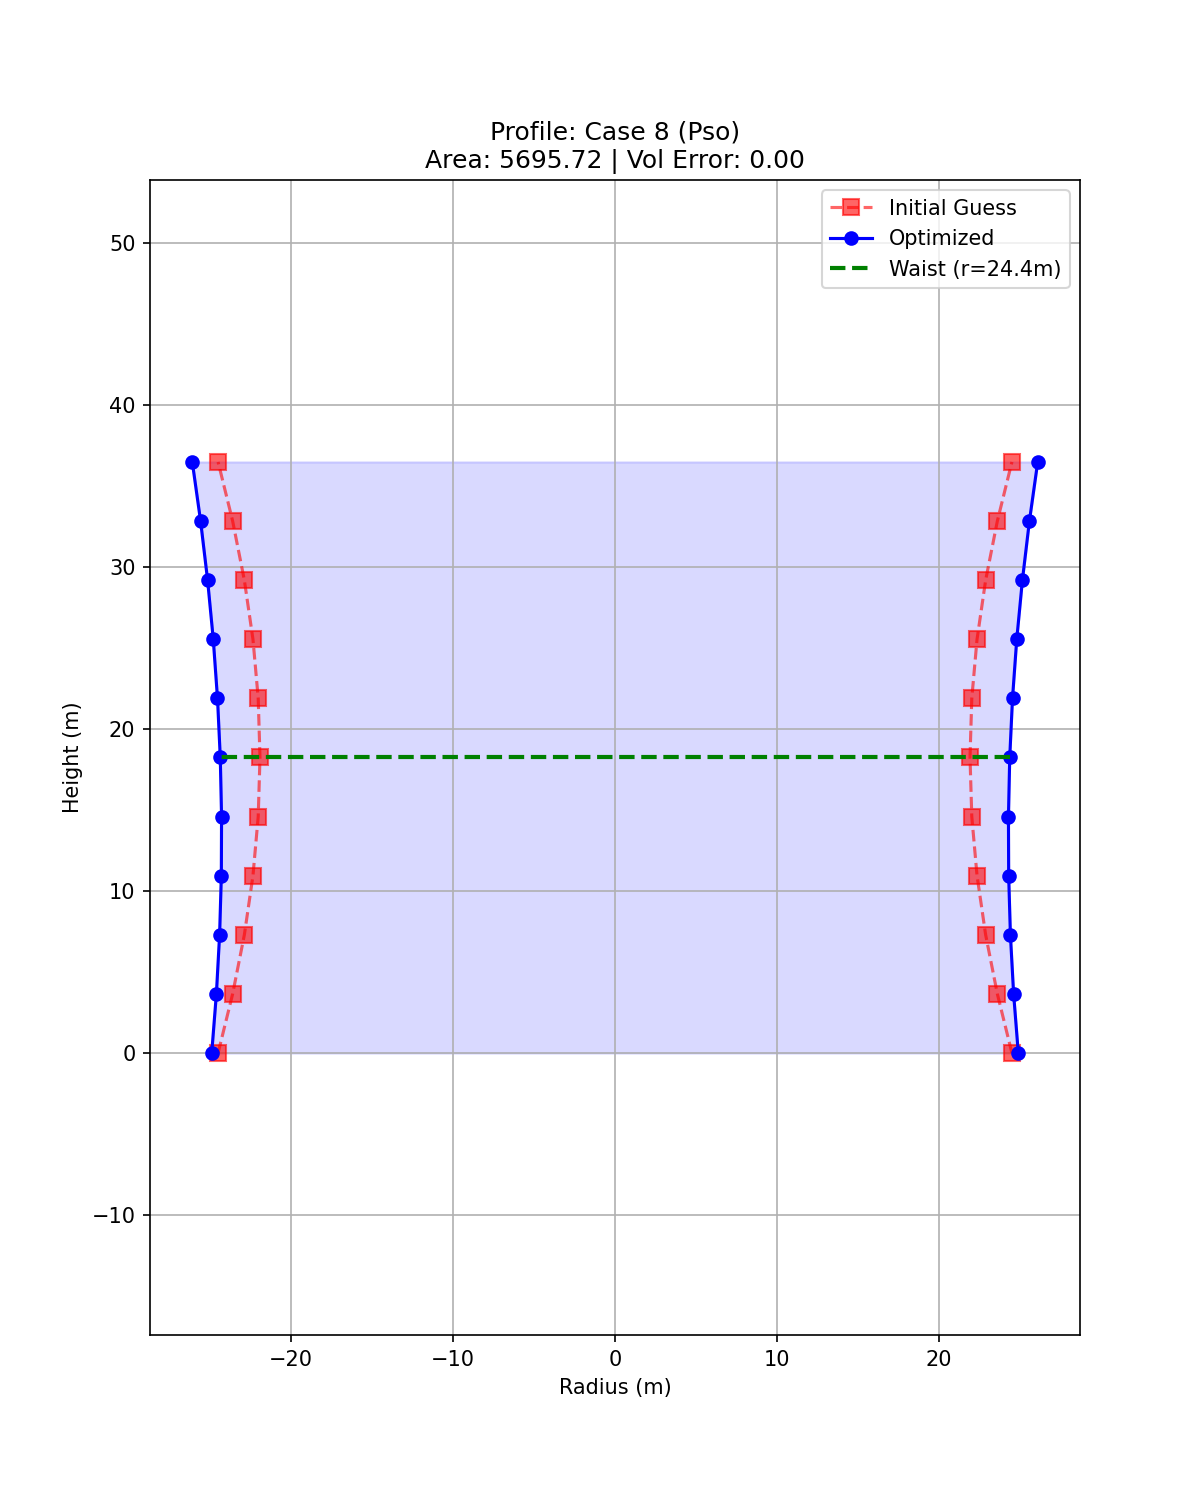
\includegraphics[width=0.50\textwidth]{../Images/PSO/Case8_Pso_profile.png}
    \caption{Best cooling tower with PSO algorithm}
\end{figure}

Based on these criteria, case 8 emerges as the most appropriate cooling‑tower configuration. First, in terms of volume fidelity, case 8 achieves a zero volume error, indicating a perfect match with the prescribed target without requiring compensatory geometric distortions. This level of accuracy is only shared with a small subset of cases, yet case 8 distinguishes itself among them through superior performance on several other dimensions.
Regarding convergence behaviour, case 8 presents one of the cleanest and most rapid convergence histories. The cost function drops sharply within the first iterations and stabilises immediately, showing no signs of late oscillations or prolonged refinement phases. This stable behaviour provides confidence in the robustness of the obtained optimum and reduces the likelihood that the solution is sensitive to stochastic fluctuations. By contrast, some alternative cases with good volume fidelity exhibit longer convergence trajectories or more gradual plateauing, which weakens their comparative reliability.
The area measure also strongly supports the selection of case 8. It yields the smallest external envelope across all eight cases, significantly lower than those of the other zero‑error candidates. As area is used here as a proxy for material and fabrication efficiency, a reduced surface envelope implies a more economical and structurally lightweight design. This advantage is particularly striking when compared with cases 1 and 5, which, despite their excellent volume match, present substantially larger envelopes.
Finally, the geometric plausibility of the resulting cooling‑tower profile reinforces this choice. The optimised shape of  case 8 is smooth, coherent, and free of abrupt curvature transitions, exhibiting a compact silhouette with a consistent radial gradient and a physically realistic waist. Among all the profiles, it is one of the most regular and least distorted, requiring only modest adjustments from the initial guess while still achieving perfect volume compliance.
Taken together, these observations show that case 8 offers the best balance of accuracy, stability, efficiency, and physical credibility. It therefore represents the most defensible choice for the optimal cooling‑tower configuration within the scope of this study.

\subsection{SA}

\subsection{BFGS}

\subsection{Global discussion}

		\pagebreak
		
		\section{Conclusion}

\subsection{Conclusion on Simulated Annealing}

The Simulated Annealing algorithm demonstrated robust performance across the eight cooling tower optimisation scenarios, consistently satisfying the volume constraint with errors below 0.5\,m$^3$ in all cases and confirming the effectiveness of the penalty-based approach.

In terms of solution quality, Case~8 (Hyperbolic Fit) achieved the minimum surface area of 5\,765.62\,m$^2$, representing a 26\% reduction compared to the reference case and highlighting the advantage of parametric formulations that reduce the search space dimension while guaranteeing physically realistic geometries. The convergence behaviour across all cases exhibited characteristic staircase patterns, with most improvements occurring within the first 2\,000 iterations; the algorithm successfully escaped local minima in early stages due to the high initial temperature. Sensitivity to initial conditions was observed in Case~5 (Cylindrical Start), where the deliberately poor starting point led to a 2.3\% increase in area compared to the reference case, indicating that SA's final solution retains some dependence on the initialisation despite its stochastic exploration mechanism. The most significant limitation emerged in Case~6 (High Volume), where the absence of explicit geometric constraints---monotonicity, convexity---allowed the SA to produce unrealistic zigzag profiles. This confirms that penalty functions alone are insufficient for shape optimisation problems requiring smooth geometries.

In summary, SA is well-suited for cooling tower optimisation when combined with appropriate geometric constraints or parametric formulations. The computational cost remains low (1.6--6.2\,s per case), making it practical for engineering design applications.

\subsection{Conclusion on Particle Swarm Optimisation}

The PSO algorithm exhibited strong exploration capabilities and reliable constraint satisfaction across all eight cases under the penalty-based formulation used in this study. Volume errors remained below 1.2\,m$^3$ in all cases, confirming that the penalty weight $\rho = 10^5$ is sufficient to guide the swarm toward the feasible manifold. However, PSO consistently produced larger surface areas than BFGS, indicating that while the swarm successfully satisfies the volume constraint, it lacks the local refinement precision required to minimise the objective function effectively.

The best performance was achieved on Case~8 (Hyperbolic Fit), which produced the lowest surface area of all algorithm--case combinations (5\,742.55\,m$^2$) with near-zero volume error, confirming that the low-dimensional parametric space enables effective swarm convergence. The two-phase convergence pattern---rapid descent followed by plateau---was consistently observed, with Cases~2, 6, and~8 converging within 30--50 iterations while Cases~1, 3, and~5 required over 500 iterations. The computational cost constitutes the most significant limitation of PSO as deployed in this study: PSO required on average 133\,800 function evaluations per case---$14\times$ more than BFGS and $8\times$ more than SA---yet produced larger surface areas than BFGS in seven out of eight cases, yielding a poor cost-effectiveness ratio that limits PSO's suitability for problems where function evaluations are expensive.

In summary, PSO's global exploration capability ensures reliable constraint satisfaction but proves insufficient to compete with gradient-based methods in terms of solution quality and computational efficiency. Future work should investigate local refinement strategies, adaptive inertia schedules, or hybrid PSO--BFGS approaches to address the precision gap observed in this study.

\subsection{Conclusion on BFGS}

The BFGS quasi-Newton method emerged as the most effective algorithm in this study, achieving the best or near-best surface area in seven out of eight cases with perfect volume constraint satisfaction (zero error in all cases) and the lowest computational cost.

Its peak performance was observed on Case~8 (Hyperbolic Fit), where BFGS converged in just 12 iterations (0.04\,s) to an area of 5\,961.77\,m$^2$ with zero volume error---the most efficient configuration in the entire study. Across all well-conditioned cases, BFGS exhibited superlinear convergence, with typical convergence achieved within 20--30 iterations; the gradient norm provides a natural, adaptive stopping criterion, in contrast to SA, which relies on a fixed iteration budget, and PSO, which terminates adaptively based on swarm stagnation. The geometric quality of the BFGS solutions was consistently superior: in Case~6 (High Volume), BFGS achieved a 4.7$\times$ lower surface area than SA, attributable entirely to the inherent geometric regularity of gradient-based search. The principal limitation was observed in Case~3 (Full Freedom, $D = 19$), where the method's vulnerability to ill-conditioning and local trapping in high-dimensional spaces led to convergence at a physically unrealistic local minimum. For such problems, BFGS should be combined with multi-start strategies or hybridised with a global search phase.

In summary, BFGS is the recommended algorithm for cooling tower optimisation when gradient information is available and the search space is well conditioned. Its deterministic nature, adaptive termination, and inherent geometric smoothness make it ideally suited for structural engineering applications where solution quality, reproducibility, and computational efficiency are paramount.

\subsection{Overall Conclusion}

This study benchmarked three optimisation algorithms---BFGS, Simulated Annealing, and Particle Swarm Optimisation---on the structural surface area minimisation of a discretised hyperboloidal cooling tower across eight study cases of increasing complexity. The investigation reveals a clear performance hierarchy: BFGS $>$ SA $\gg$ PSO, with the following overarching conclusions:

\begin{enumerate}
    \item \textbf{Algorithm selection matters, but problem formulation matters more.} Case~8 (Hyperbolic Parametrisation, $D = 3$) yielded the best result for all three methods, demonstrating that embedding physical knowledge into the parametrisation is more effective than algorithmic sophistication.
    
    \item \textbf{Gradient-based methods are naturally suited to shape optimisation.} BFGS's local search produces smooth, structurally plausible profiles without requiring explicit geometric penalties, whereas stochastic methods can generate unrealistic geometries unless additional constraints are imposed.
    
    \item \textbf{Penalty-based constraint handling is effective across all three methods.} The static penalty weight $\rho = 10^5$ is sufficient to guide all three algorithms toward the feasible manifold, with volume errors below 1.2\,m$^3$ for PSO, below 0.75\,m$^3$ for SA, and zero for BFGS in seven out of eight cases. However, PSO's distributed evaluation strategy limits its ability to exploit local curvature near the feasible manifold, suggesting that a hybrid penalty--refinement approach would improve surface area precision.
    
    \item \textbf{Computational efficiency spans three orders of magnitude.} BFGS achieves convergence in $\mathcal{O}(10^2)$ function evaluations, SA in $\mathcal{O}(10^4)$, and PSO in $\mathcal{O}(10^5)$, with BFGS delivering superior solutions at the lowest cost in the majority of cases.
\end{enumerate}

\subsection{Future Work}

Building on the limitations identified in Section~5.4.4, several directions for future investigation are proposed:

\begin{itemize}
    \item \textbf{Constraint handling}: As noted in the limitations discussion, the penalty weight $\rho = 10^5$ is suboptimal for the stochastic methods. Future work should investigate augmented Lagrangian methods, feasibility-preserving operators for PSO, and adaptive penalty schedules to improve performance on equality-constrained problems.
    
    \item \textbf{Hybrid algorithms}: Combine global exploration (SA or PSO) with local refinement (BFGS) in a two-phase strategy, using the stochastic method to identify promising basins and BFGS to converge within them.
    
    \item \textbf{Structural constraints}: Extending the cost function to incorporate stress, buckling, and wind-load criteria---identified in Section~5.4.4 as a key omission of the present study---would transform the problem into a multi-objective optimisation that more closely reflects real engineering requirements.
    
    \item \textbf{Higher-fidelity models}: Replace the conical frustum discretisation with finite element shell models to capture bending stiffness, membrane stress distributions, and nonlinear geometric effects.
    
    \item \textbf{Parametric exploration}: Investigate alternative parametric families beyond the hyperboloid of one sheet (e.g., polynomial profiles, B-spline representations) to assess whether further surface area reductions are achievable while maintaining structural integrity.
\end{itemize}

		\pagebreak
		
		\printbibliography[heading=bibintoc, title={References}]
		\pagebreak
		
		\clearpage

\section{Appendices}

% \appendix to change numbering to A, B, C for subsections
\appendix

% Renew section commands to show "Appendix A", "Appendix A.A" format
\renewcommand{\thesubsection}{Appendix \Alph{subsection}}
\renewcommand{\thesubsubsection}{Appendix \Alph{subsection}.\Alph{subsubsection}}

\subsection{Code Listings}

\subsubsection{PSO implementation}

TO DO

\subsubsection{SA implementation}

TO DO

\subsubsection{BFGS implementation}

TO DO

\subsection{Detailed Results Data}

\subsubsection{PSO results}

TO DO

\subsubsection{SA results}

TO DO

\subsubsection{BFGS results}

TO DO
		\pagebreak
	}
\end{document}